\title{%
  DD1301 Datorintroduktion
}
\author{Daniel Bosk}
\institute{%
  KTH EECS
}

\mode<article>{\maketitle}
\mode<presentation>{%
  \begin{frame}
    \maketitle
  \end{frame}
}

\mode*


\section{Terminal}

\begin{frame}[fragile]
  \begin{lstlisting}[numbers=none]
n=10 cat hitch-hikers-guide.txt | \
  tr -cs A-Za-z '\n' | tr A-Z a-z | \
  sort | \
  uniq -c | \
  sort -rn | \
  head -n \$n
  \end{lstlisting}
\end{frame}


\section{Version management}

\begin{frame}
  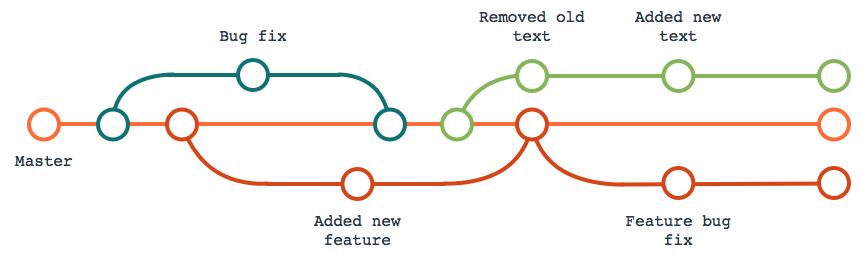
\includegraphics[width=\columnwidth]{version-tree.png}
\end{frame}


\section{\LaTeX}

\begin{frame}
\[
  R = \left(\argmin_{\substack{RR^t=I,\\ \det(R)=1}}
  \sum_{i=1}^n \omega_i 
\norm{RX_i-Y_i}^2_2\right)^{{L}{\sqrt{1-\frac{v^2}{c^2}}}},
\]

%  \begin{lstlisting}
%R^*=\argmin_{\substack{RR^t=I,\\ \det(R)=1}}
%    \sum_{i=1}^n \omega_i \norm{RX_i-Y_i}^2_2,
%  \end{lstlisting}
\end{frame}

\begin{frame}[fragile]
  \lstinputlisting[firstline=19,firstnumber=19,lastline=37]{contents.tex}
\end{frame}


%%% REFERENCES %%%

\begin{frame}[allowframebreaks]
  \printbibliography{}
\end{frame}
